\documentclass[12pt]{amsart}

\usepackage{amsmath,amssymb,amsfonts,amsthm}
\usepackage{enumerate}
\usepackage{eucal}
\usepackage{graphicx,psfrag}
\usepackage{ifthen}

% Margins and spacing
\evensidemargin 0.1 in \oddsidemargin 0.1 in
\parindent 24pt
\textheight 9.6 in \textwidth 6.2 in
\baselineskip 9.6 in \topmargin 0.005 in

% Line spacing
\newcommand{\Normalstretch}{1.0}
\renewcommand{\baselinestretch}{\Normalstretch}
\newenvironment{singlespace}
{\renewcommand{\baselinestretch}{1} \small \normalsize}
{\renewcommand{\baselinestretch}{\Normalstretch} \small \normalsize}

% Theorem environments
\newtheorem{mydef}{Definition}
\newtheorem{thm}{Theorem}
\newtheorem{lemma}[thm]{Lemma}
\newtheorem{claim}[thm]{Claim}
\newtheorem{proposition}[thm]{Proposition}
\newtheorem{conjecture}[thm]{Conjecture}
\newtheorem{corollary}[thm]{Corollary}
\theoremstyle{remark}
\newtheorem{rmk}{Remark}[section]
\newenvironment{remark}{\begin{rmk}\rm\baseenvskip}{\end{rmk}}
\newtheorem{definition}[rmk]{Definition}

\numberwithin{equation}{section}
\numberwithin{thm}{section}
\numberwithin{rmk}{section}
\numberwithin{figure}{section}

% Shortcuts
\newcommand{\hhs}[1]{\hspace{#1mm}}
\newcommand{\hs}{\hspace{5mm}}
\newcommand{\vp}{\vspace{1mm}}
\newcommand{\vs}{\vspace{5mm}}
\newcommand{\jl}{$\frac{}{}$}
\newcommand{\mbf}[1]{\mbox{\boldmath $#1$}}
\newcommand{\hb}[1]{\hspace{-#1 mm}}
\newcommand{\ds}{\displaystyle}
\newcommand{\QED}{\hfill $\Box$}
\newcommand{\norm}[1]{\left\Vert#1\right\Vert}
\newcommand{\abs}[1]{\left\vert#1\right\vert}
\newcommand{\set}[1]{\left\{#1\right\}}
\newcommand{\N}{\mathbb{N}}
\newcommand{\Q}{\mathbb{Q}}
\newcommand{\Hv}{\mathcal{H}_v}
\newcommand{\h}{\mathcal{H}}
\newcommand{\Ov}{\mathcal{O}_v}
\newcommand{\F}{\mathcal{F}}
\newcommand{\Rn}{R^n}
\newcommand{\C}{\mathbb{C}}
\newcommand{\Ce}{\widehat{\mathbb{C}}}
\newcommand{\si}{\sigma}
\newcommand{\Cn}{\mathbb{C}^n}
\newcommand{\Z}{\mathbb{Z}}
\newcommand{\p}{\partial}
\newcommand{\ep}{\varepsilon}
\newcommand{\D}{\delta}
\newcommand{\eps}{\varepsilon}
\newcommand{\finv}{f^{-1}}
\newcommand{\im}{\imath}
\newcommand{\ga}{\gamma}
\newcommand{\ze}{\zeta}
\newcommand{\fee}{\varphi}
\newcommand{\noi}{\noindent}

\title{Q1 Maximizing Correlation}
\author{Juba Cochran}
\date{\today}

\begin{document}
\maketitle

\vspace{2em}
What are the possible values for $\rho(X,Y)$, the correlation between $X$ and $Y$? 
\vspace{2em}
\begin{definition}[2.2.5: Correlation]
The Correlation of two random variables X and Y with $\sigma[X] > 0$ and $\sigma[Y] > 0$ is:
\[
\rho(X, Y) = \frac{\text{Cov}(X, Y)}{\sigma_X \cdot \sigma_Y}
\]
\begin{thm}[2.2.6: Correlation and Linear Dependence]
For random variables $X$ and $Y$:
\begin{itemize}
    \item $\rho(X, Y) \in [-1, 1]$
    \item $\rho(X, Y) = 1 \iff \exists a, b \in \mathbb{R} \text{ with } b > 0 \text{ such that } Y = a + bX$
    \item $\rho(X, Y) = -1 \iff \exists a, b \in \mathbb{R} \text{ with } b > 0 \text{ such that } Y = a - bX$
\end{itemize}
\end{thm}

\begin{proof}
Given: $Y = aX + b$ where $a \ne 0$ and $b \in \mathbb{R}$. This is a perfect linear relationship.

Let us analyze by observing the correlation definition and using Theorem 2.2.6.

\begin{itemize}
    \item If $a > 0$, we can rewrite $Y = b + aX$ which matches the form $Y = a + bX$ with $b > 0$, so $\rho(X, Y) = 1$.
    \item If $a < 0$, we can rewrite $Y = b - |a|X$, which matches the form $Y = a - bX$ with $b > 0$, so $\rho(X, Y) = -1$.
\end{itemize}

Therefore, the only possible values of $\rho(X, Y)$ in this case are:
\[
\pm 1
\]

\begin{figure}[h]
    \centering
    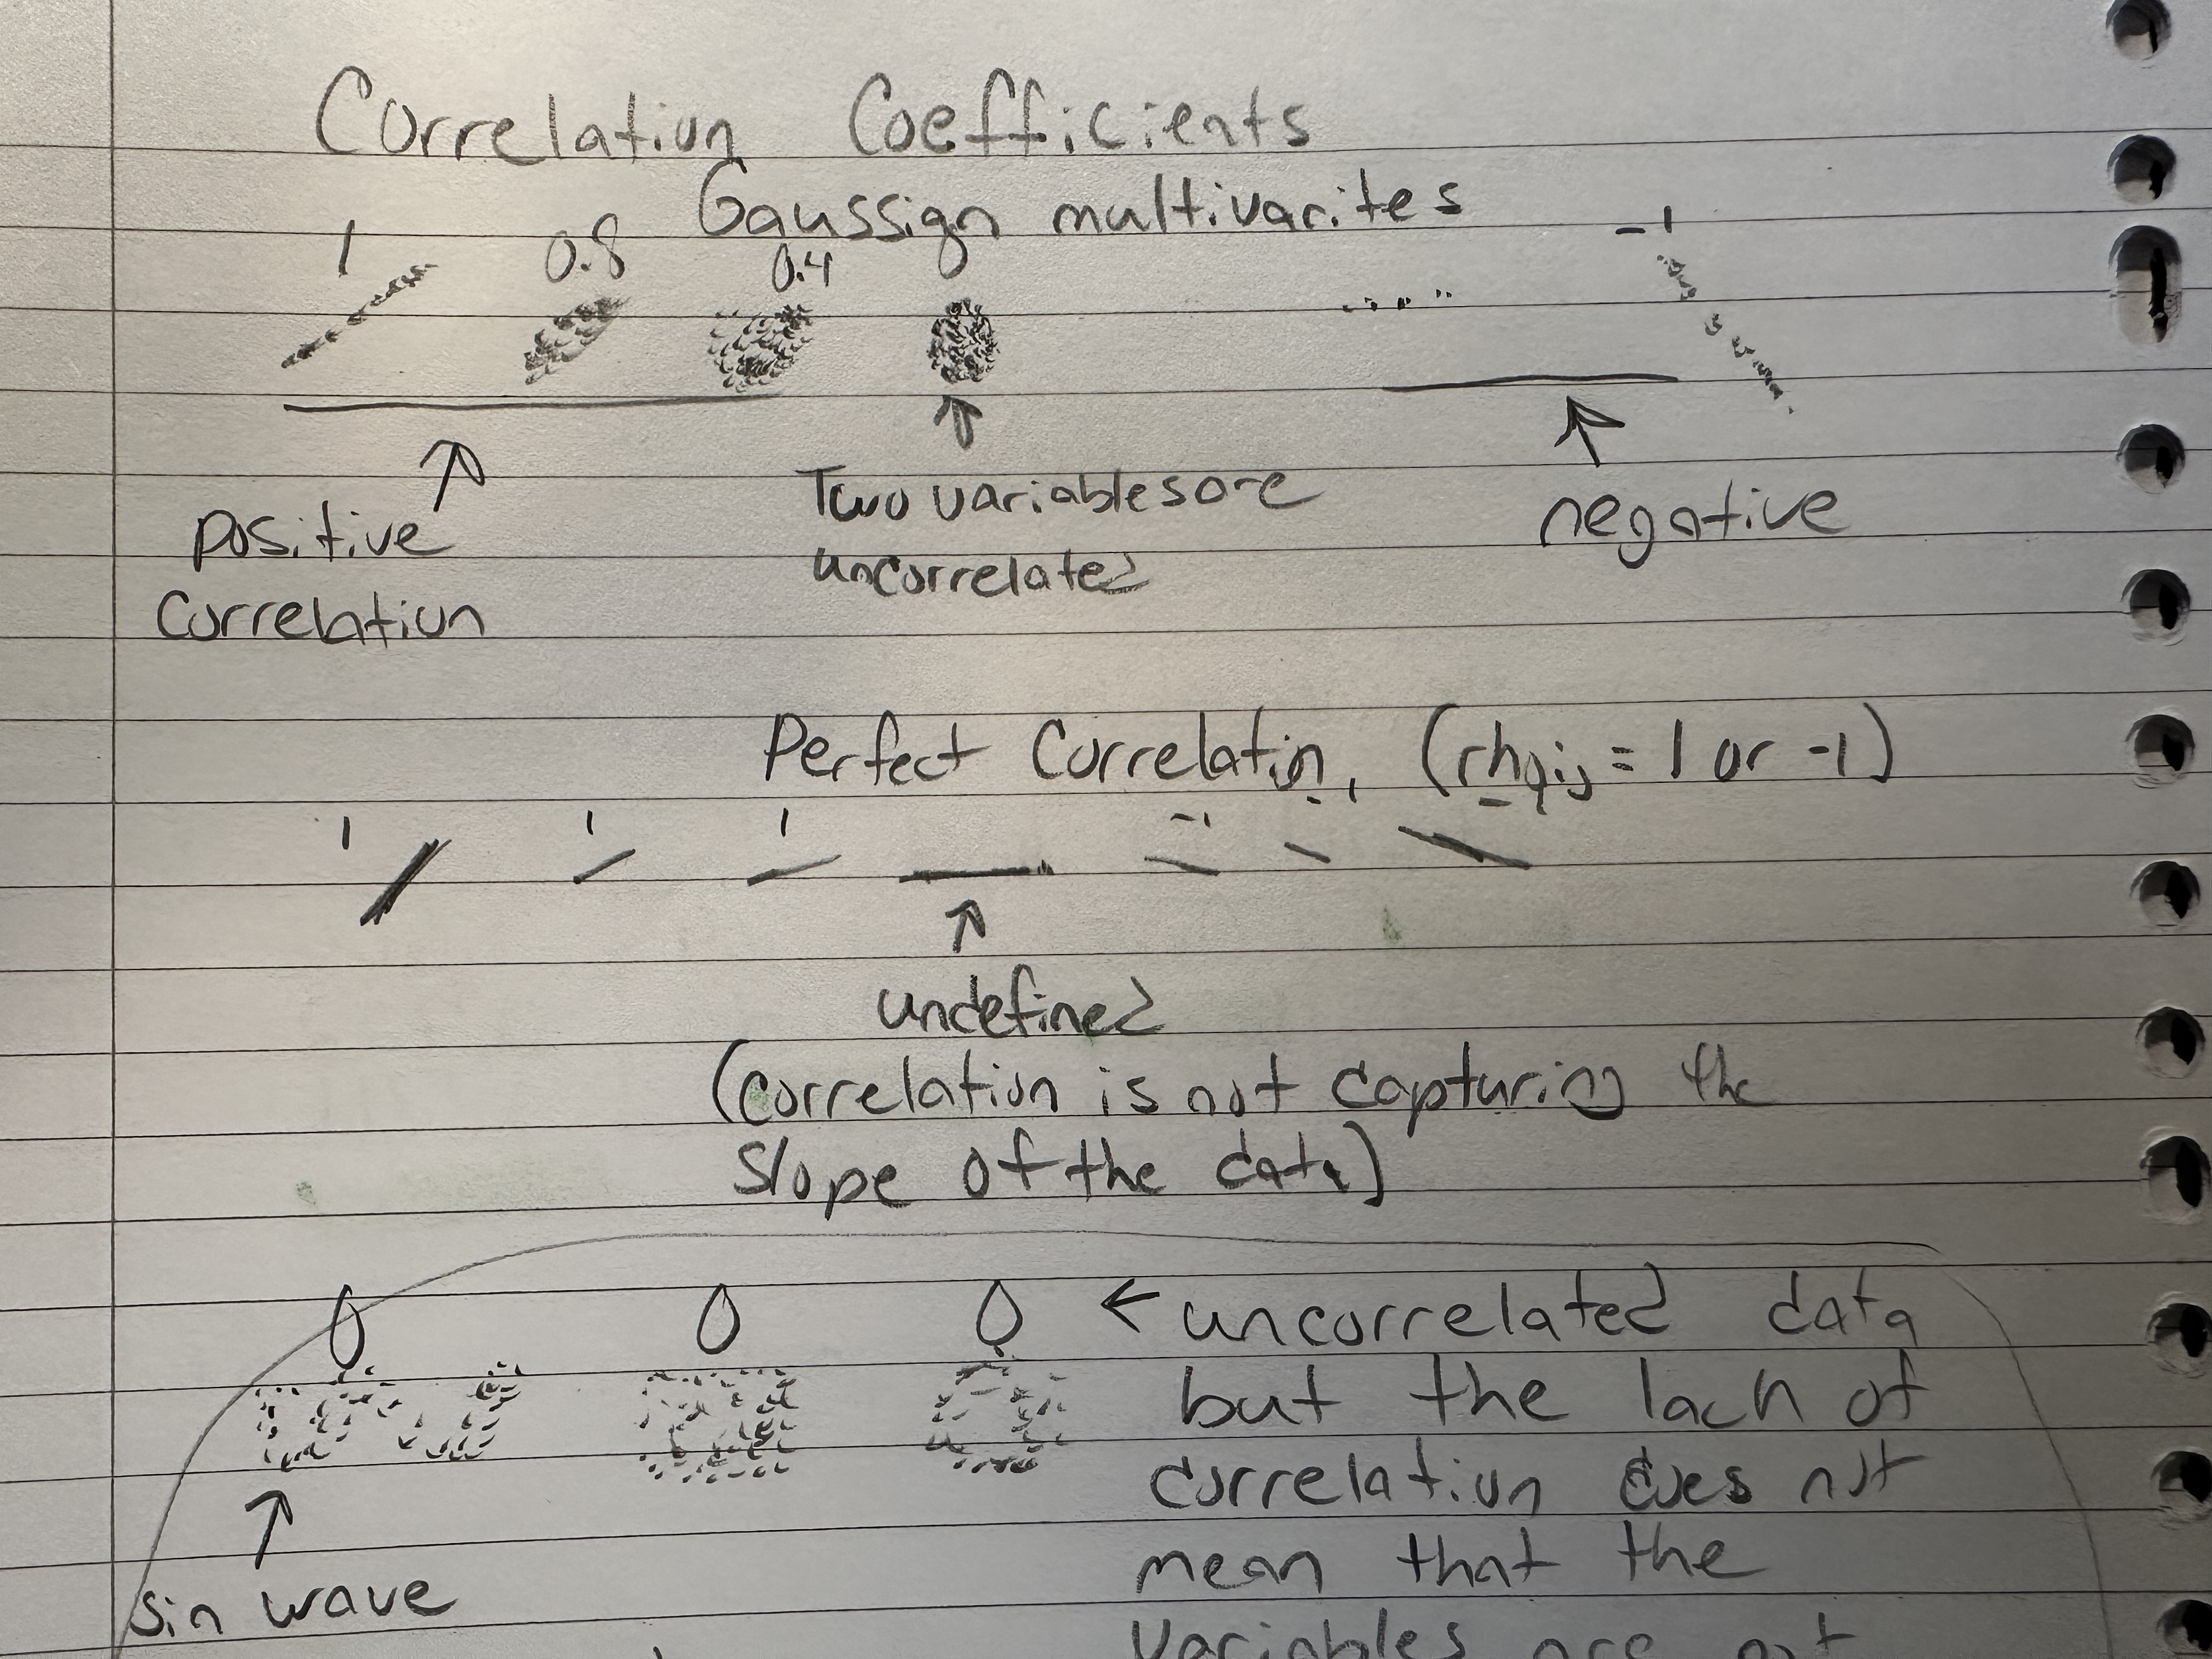
\includegraphics[width=0.9\textwidth]{IMG_7685.JPG}
    \caption{Personal Hand-drawn illustrations of correlation coefficients, including positive, negative, zero, and nonlinear cases.}
    \label{fig:correlation-sketch}
\end{figure}

\end{proof}

\end{document}